\documentclass{report}
% Include all project wide packages here.
\usepackage{fullpage}
\usepackage[style=ieee]{biblatex}
\usepackage[dutch]{babel}

\renewcommand{\familydefault}{\sfdefault}

\setmainfont[Ligatures=TeX]{Myriad Pro}
\setmathfont{Asana Math}
\setmonofont{Lucida Console}

\usepackage{titlesec, blindtext, color}
\definecolor{gray75}{gray}{0.75}
\newcommand{\hsp}{\hspace{20pt}}
\titleformat{\chapter}[hang]{\Huge\bfseries}{\thechapter\hsp\textcolor{gray75}{|}\hsp}{0pt}{\Huge\bfseries}
\renewcommand{\familydefault}{\sfdefault}
\renewcommand{\arraystretch}{1.2}
\setlength\parindent{0pt}

%For code listings
\definecolor{black}{rgb}{0,0,0}
\definecolor{browntags}{rgb}{0.65,0.1,0.1}
\definecolor{bluestrings}{rgb}{0,0,1}
\definecolor{graycomments}{rgb}{0.4,0.4,0.4}
\definecolor{redkeywords}{rgb}{1,0,0}
\definecolor{bluekeywords}{rgb}{0.13,0.13,0.8}
\definecolor{greencomments}{rgb}{0,0.5,0}
\definecolor{redstrings}{rgb}{0.9,0,0}
\definecolor{purpleidentifiers}{rgb}{0.01,0,0.01}


\lstdefinestyle{csharp}{
language=[Sharp]C,
showspaces=false,
showtabs=false,
breaklines=true,
showstringspaces=false,
breakatwhitespace=true,
escapeinside={(*@}{@*)},
columns=fullflexible,
commentstyle=\color{greencomments},
keywordstyle=\color{bluekeywords}\bfseries,
stringstyle=\color{redstrings},
identifierstyle=\color{purpleidentifiers},
basicstyle=\ttfamily\small}

\lstdefinestyle{c}{
language=C,
showspaces=false,
showtabs=false,
breaklines=true,
showstringspaces=false,
breakatwhitespace=true,
escapeinside={(*@}{@*)},
columns=fullflexible,
commentstyle=\color{greencomments},
keywordstyle=\color{bluekeywords}\bfseries,
stringstyle=\color{bluestrings},
identifierstyle=\color{purpleidentifiers}
}

\lstdefinestyle{vhdl}{
language=VHDL,
showspaces=false,
showtabs=false,
breaklines=true,
showstringspaces=false,
breakatwhitespace=true,
escapeinside={(*@}{@*)},
columns=fullflexible,
commentstyle=\color{greencomments},
keywordstyle=\color{bluekeywords}\bfseries,
stringstyle=\color{redstrings},
identifierstyle=\color{purpleidentifiers}
}

\lstdefinestyle{xaml}{
language=XML,
showspaces=false,
showtabs=false,
breaklines=true,
showstringspaces=false,
breakatwhitespace=true,
escapeinside={(*@}{@*)},
columns=fullflexible,
commentstyle=\color{greencomments},
keywordstyle=\color{redkeywords},
stringstyle=\color{bluestrings},
tagstyle=\color{browntags},
morestring=[b]",
  morecomment=[s]{<?}{?>},
  morekeywords={xmlns,version,typex:AsyncRecords,x:Arguments,x:Boolean,x:Byte,x:Char,x:Class,x:ClassAttributes,x:ClassModifier,x:Code,x:ConnectionId,x:Decimal,x:Double,x:FactoryMethod,x:FieldModifier,x:Int16,x:Int32,x:Int64,x:Key,x:Members,x:Name,x:Object,x:Property,x:Shared,x:Single,x:String,x:Subclass,x:SynchronousMode,x:TimeSpan,x:TypeArguments,x:Uid,x:Uri,x:XData,Grid.Column,Grid.ColumnSpan,Click,ClipToBounds,Content,DropDownOpened,FontSize,Foreground,Header,Height,HorizontalAlignment,HorizontalContentAlignment,IsCancel,IsDefault,IsEnabled,IsSelected,Margin,MinHeight,MinWidth,Padding,SnapsToDevicePixels,Target,TextWrapping,Title,VerticalAlignment,VerticalContentAlignment,Width,WindowStartupLocation,Binding,Mode,OneWay,xmlns:x}
}

%defaults
\lstset{
basicstyle=\ttfamily\small,
extendedchars=false,
numbers=left,
numberstyle=\ttfamily\tiny,
stepnumber=1,
tabsize=4,
numbersep=5pt
}
\title{Resultaten}
\author{J.F.J. Blom}
\date{\today}
\begin{document}
\chapter{Resultaten en Discussie}
Er zijn vier verschillende metingen verricht, kalibratiemeting, onbekende afstandsmeting en de lineariteitsmeting. In dit hoofstuk zijn alle meetresultaten weergeven en geanalyseerd.Van alle meetresultaten is het gemiddelde genomen, doormiddel van deze formule:
\begin{equation}
\frac{\sum_{i=1}^{n}x_i}{n}
\end{equation}

Hier is $x_i$ een meetresultaat en n is het aantal metingen. 
Daarnaast is de onzekerheid van de metingen berekend. Daarbij is gebruik gemaakt van de volgende formule:
\begin{equation}
\sqrt{\frac{\sum_{i=1}^{n}( x_i-x_a)^2}{n(n-1)}}
\end{equation}
$x_a$ is hier het gemiddelde van de meting.
\subsection*{Kalibratie}
Hieronder zijn de meetresultaten van de kalibratiemeting te zien. De meetresultaten zijn vrij constant, en dus is de onzekerheid vrij laag. De onzekerheid van de tijdsmeting is vastgesteld op 0.003 seconden, waaruit blijkt dat de meting erg accuraat is. De onzekerheid van de snelheid wordt dan 0.025 cm/s. De gemiddelde snelheid is ongeveer 9.6 cm/s.

\begin{table}
 \centering
\begin{tabular}{| l| c|}
\hline
    & Kalibratie 10 cm \\
\hline
   Meting 1 (s) & 1.031 \\
\hline
   Meting 2 (s) & 1.042 \\
\hline
   Meting 3 (s) & 1.042 \\
\hline
   Meting 4 (s) & 1.046 \\
\hline
   Meting 5 (s) & 1.045 \\
\hline
   Gemiddelde (s) & 1.041 \\
\hline
   Gemiddelde snelheid (cm/s) & 9.602 \\
\hline
   Onzekerheid tijd (s) & 0.003 \\
\hline
   Onzekerheid snelheid (cm/s) & 0.025 \\
\hline
\end{tabular}
\caption{Tabel meetresultaten kalibratie Joris en Chy}
\end{table}

\begin{table}
 \centering
\begin{tabular}{| l| c|}
\hline
    & Kalibratie 10 cm \\
\hline
   Meting 1 (s) & 1,164 \\
\hline
   Meting 2 (s) & 1.170 \\
\hline
   Meting 3 (s) & 1.173 \\
\hline
   Meting 4 (s) & 1.142 \\
\hline
   Meting 5 (s) & 1.146 \\
\hline
   Meting 6 (s) & 1.167 \\
\hline
   Meting 7 (s) & 1.171 \\
\hline
   Meting 8 (s) & 1.167 \\
\hline
   Meting 9 (s) & 1.156 \\
\hline
   Meting 10 (s) & 1.152 \\
\hline
   Gemiddelde (s) & 1.161 \\
\hline
   Gemiddelde snelheid (cm/s) & 8.614 \\
\hline
   Onzekerheid tijd (s) & 1.208E-5
 \\
\hline
   Onzekerheid snelheid (cm/s) & 1.040E-4 \\
\hline
\end{tabular}
\caption{Tabel meetresultaten kalibratie Luc en Tijmen}
\end{table}

\begin{figure}[H]
 \centering
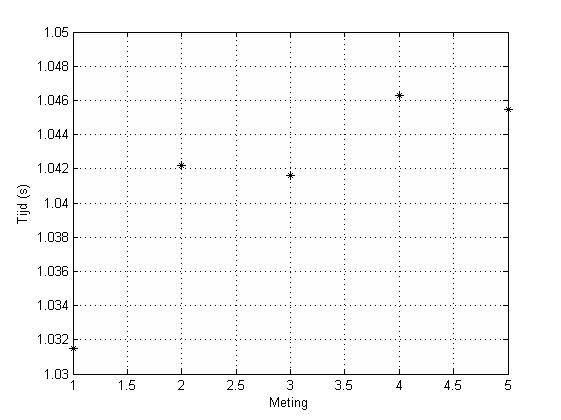
\includegraphics[width=150mm] {grafiekmeetresultaten.jpg}
\caption{Grafiek meetresultaten kalibratie Joris en Chy}
\end{figure}
Hierboven zijn de meetresultaten van de kalibratiemeting in een diagram gezet. Hier zijn goed de verschillen tussen de metingen te zien. De metingen liggen redelijk dicht bij elkaar, en dus is de kwaliteit van deze meting erg hoog.
\section{Onbekende afstand}
Hieronder zijn de meetresultaten te zien van de onbekende afstandsmeting. Om de snelheid te kunnen bepalen moet er een afstand bekend zijn. Deze afstand is gemeten en deze is 23.4 cm. De onzekerheid van de tijdsmeting is vastgesteld op 0.005 seconden, en dus is de meting erg nauwkeurig. Deze meting is zoals verwacht vanwege de langere afstand iets minder accuraat als de kalibratiemeting. De onzekerheid van de snelheid is vastgesteld op 0.007 cm/s, en dus is ook deze waarde erg nauwkeurig. De snelheid is zoals verwacht ongeveer gelijk als bij de kalibratiemeting.

\begin{table}
 \centering
\begin{tabular}{| l| c|}
\hline
    & Onbekende afstand 23.4 cm\\
\hline
   Meting 1 (s) & 2.526 \\
\hline
   Meting 2 (s) & 2.531 \\
\hline
   Meting 3 (s) & 2.515 \\
\hline
   Meting 4 (s) & 2.518 \\
\hline
   Meting 5 (s) & 2.522 \\
\hline
   Gemiddelde (s) & 2.523 \\
\hline
   Gemiddelde snelheid (cm/s) & 9.276 \\
\hline
   Onzekerheid tijd (s) & 0.005 \\
\hline
   Onzekerheid snelheid (cm/s) & 0.007 \\
\hline
 \end{tabular}
\caption{TODO caption}
\end{table}

\section{Lineariteit}
Hieronder zijn de meetresultaten te zien van de lineariteitsmeting. Doormiddel van de meetresultaten en de afstand is de gemiddelde snelheid uitgerekend. Zoals in de tabel te zien is blijft de gemiddelde snelheid redelijk constant. Dit betekend dat de afstandsmeter van de robot redelijk lineair is. De snelheid is ook ongeveer gelijk als bij de kalibratiemeting. Onder de tabel en op de volgende pagina zijn deze gegevens in diagrammen gezet, waardoor de afwijkingen in lineariteit nog beter te zien zijn. 

\begin{table}
 \centering
\begin{tabular}{| l| c| c| c| c| c|}
\hline
   & 5 cm & 10 cm & 15 cm & 20 cm & 25 cm\\
\hline
   Meting 1 (s) & 0.542 & 1.092 & 1.638 & 2.218 & 2.728 \\
\hline
   Meting 2 (s) & 0.550 & 1.086 & 1.636 & 2.237 & 2.747 \\
\hline
   Meting 3 (s) & 0.547 & 1.089 & 1.627 & 2.210 & 2.728 \\
\hline
   Meting 4 (s) & 0.548 & 1.081 & 1.634 & 2.218 & 2.724 \\
\hline
   Meting 5 (s) & 0.542 & 1.081 & 1.658 & 2.233 & 2.733 \\
\hline
   Gemiddelde (s) & 0.546 & 1.086 & 1.638 & 2.223 & 2.732 \\
\hline
   Gemiddelde snelheid (cm/s) & 9.164 & 9.211 & 9.155 & 8.996 & 9.151 \\
\hline
   Onzekerheid tijd (s) & 0.002 & 0.002 & 0.005 & 0.005 & 0.004 \\
\hline
   Onzekerheid snelheid (cm/s) & 0.055 & 0.018 & 0.019 & 0.10 & 0.005 \\
\hline
 \end{tabular}
\caption{TODO caption}
\end{table}
\begin{figure}[H]
 \centering
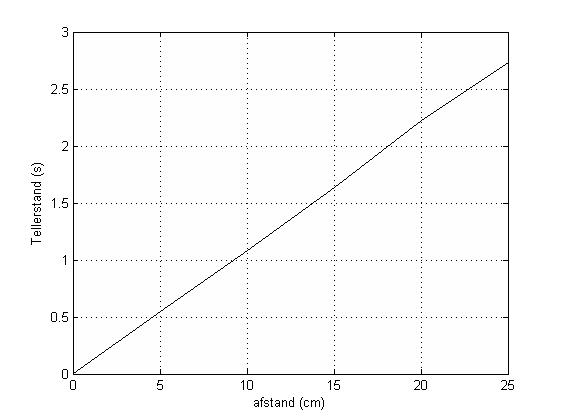
\includegraphics[width=150mm] {afstand-tellerstand.jpg}
\caption{TODO Caption}
\end{figure}
In de bovenstaande grafiek is de afstand afgezet tegen de tellerstand van de robot. De lijn is bijna recht, dus de afstandsmeter van de robot is ook bijna lineair, en dus is de snelheid onafhankelijk van de afstand.  Op de volgende pagina zet ik de afstand af tegen de snelheid, waardoor de afwijkingen in lineariteit beter te zien zijn. 
\begin{figure}[H]
 \centering
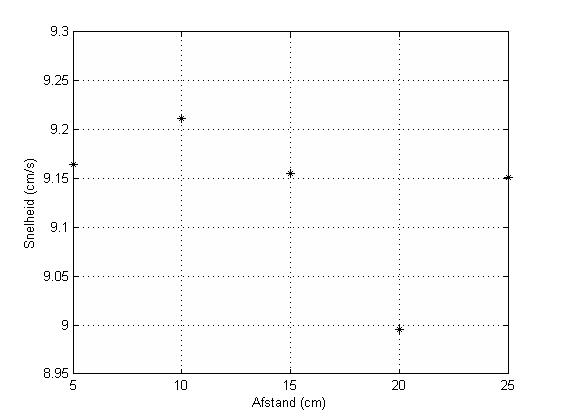
\includegraphics[width=150mm] {afstand-snelheid.jpg}
\caption{TODO Caption}
\end{figure}
In de bovenstaande grafiek is de afstand afgezet tegen de snelheid. Hier zijn goed de afwijkingen in lineariteit van de afstandsmeter te zien. De snelheid blijft tussen de 9.22 en de 8.99, dus de snelheid is vrij constant. De afstandsmeter van de robot is dus behoorlijk lineair. De kleine afwijkingen kunnen ook liggen aan de vele andere factoren die de meting be"invloeden. De robot rijd bijvoorbeeld in een bocht met een radius van 80 cm. Daarnaast is de robot misschien niet altijd loodrecht ten opzichte van de startlijn gestart, waardoor de meting wordt be"invloed.
\newpage
\chapter{Conclusie}
Het meetresultaat van dit meetrapport is goed te gebruiken in de rest van ons project. Dit is mede te danken aan de hoge kwaliteit van de meetresultaten. De onzekerheid en de afwijkingen zijn erg klein bij alle metingen die zijn verricht. De gemiddelde snelheid van de robot is ongeveer 9,6 cm/s. Bij de lineariteitsmeting was de gemiddelde snelheid vrijwel onafhankelijk van de afstand, en dus is de afstandsmeter van de robot erg lineair. Tijdens het rijden maakt de robot een bocht met een radius van ongeveer 80 cm. Hiermee moet rekening gehouden worden bij het programmeren van de robot. Het feit dat de afstandsmeter van de robot erg lineair is, is een gunstige conclusie voor ons project.
\end{document}